The purpose of this case is to test the computation of the loss exceedance probabilities when the time period associated with the loss curve calculation is different from the time period associated with the hazard curve calculation. In this case, each stochastic event set in the hazard calculation spans a time period of $t_H = $50 years, and the loss curve is calculated for a time period of $t_R = $75 years. The number of stochastic event sets (SES) used in this case is 20,000. The number of SES and $t_H$ are employed in obtaining the annual loss exceedance rates or frequencies from the ELT, and $t_R$ is employed as described in Equation~\ref{eqn:ebr-rate-to-prob} to convert back from rates of exceedance to probabilities of exceedance over the time period $t_R$.

Table~\ref{tab:vf-ln-tax1-nzcov} shows the mean loss ratios and corresponding coefficients of variation for the vulnerability function used in this test case.

The loss curve calculated using the implementation of the calculator in Julia is compared with that produced by OpenQuake in Figure~\ref{fig:lc-ebr-3a}.

\begin{figure}[htbp]
\centering
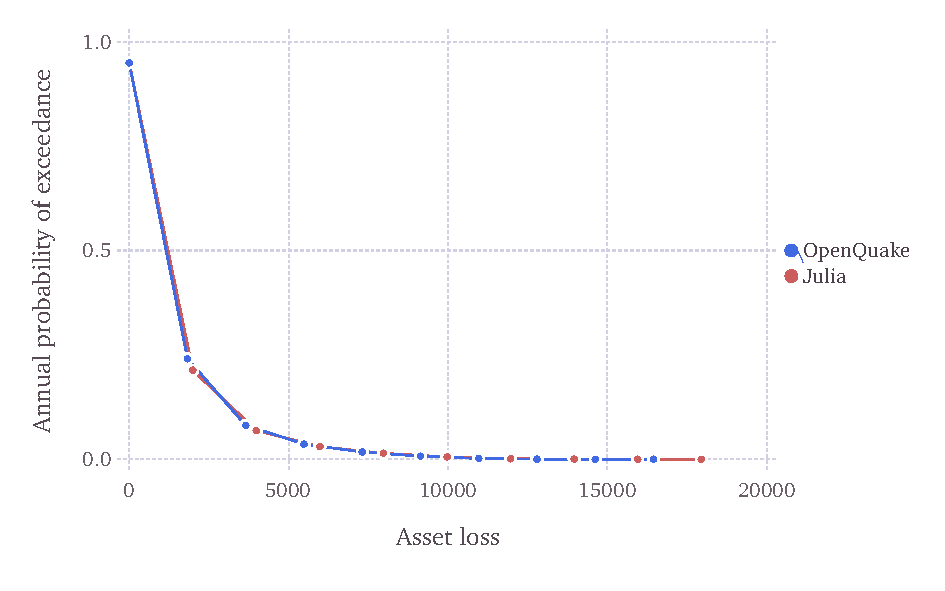
\includegraphics[width=12cm]{qareport/figures/fig-lc-ebr-3a}
\caption{Loss curve comparison for event based risk test case 3a}
\label{fig:lc-ebr-3a}
\end{figure}